% Shows the results of running our Method in the setting described in the Experimental Setup section.
% Includes reasonable comparisons and ablations so that all the claims we made in the Abstract and Intro are justified.

% MAIN CHART with killer caption (ideally this caption explains the whole paper)
% EXPLANATION


\begin{figure}[h]
    \centering
    \begin{minipage}{0.3\linewidth}
        \centering
        % If you want to frame the image, uncomment the next line and comment out the original \includegraphics line
        % \fbox{\includegraphics[width=\linewidth]{figs/figure.png}}
        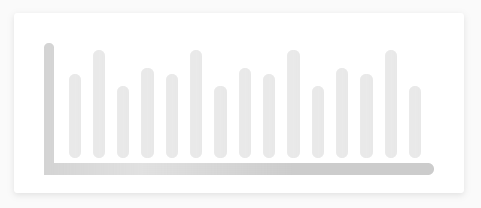
\includegraphics[width=\linewidth]{assets/chart_placeholder.png}
    \end{minipage}
    \caption{Figure clearly showing technical details of measurements made by experiments.}
    \label{fig:system}
    \end{figure}

% A set of experiments that usefully explore how good/interesting the method/model/central investigation of the paper is, and which tell a clear and cohesive story.
% Everything that appears in the Methods/Experimental Setup section should be tested, with ablations if feasible.

% We want to show absolute performance, performance relative to baselines and previous methods
% and performance compared to other methods introduced in this work and/or ablations.

% [TODO: ENTER TABLE TEMPLATE HERE]



% SUPPORTING CHARTS
% EXPLANATION
